Another useful time response of our first-order model is the response with no input ($f(t)=0$) and an initial condition ($y(0)=y_o$).  The solution to (\ref{e:first}) under these conditions is 
\begin{equation}\label{e:firstfree}
y(t) = y_o \, e^{-t/\tau}
\end{equation}
for $t>0$. Figure~\ref{f:firstfree} illustrates this free response.  Just as before the time constant is the key factor that determines the characteristic of the response.  Again, at $t=\tau$ the output has fallen by 63.2\%.
\begin{figure}[hbt]
\centering
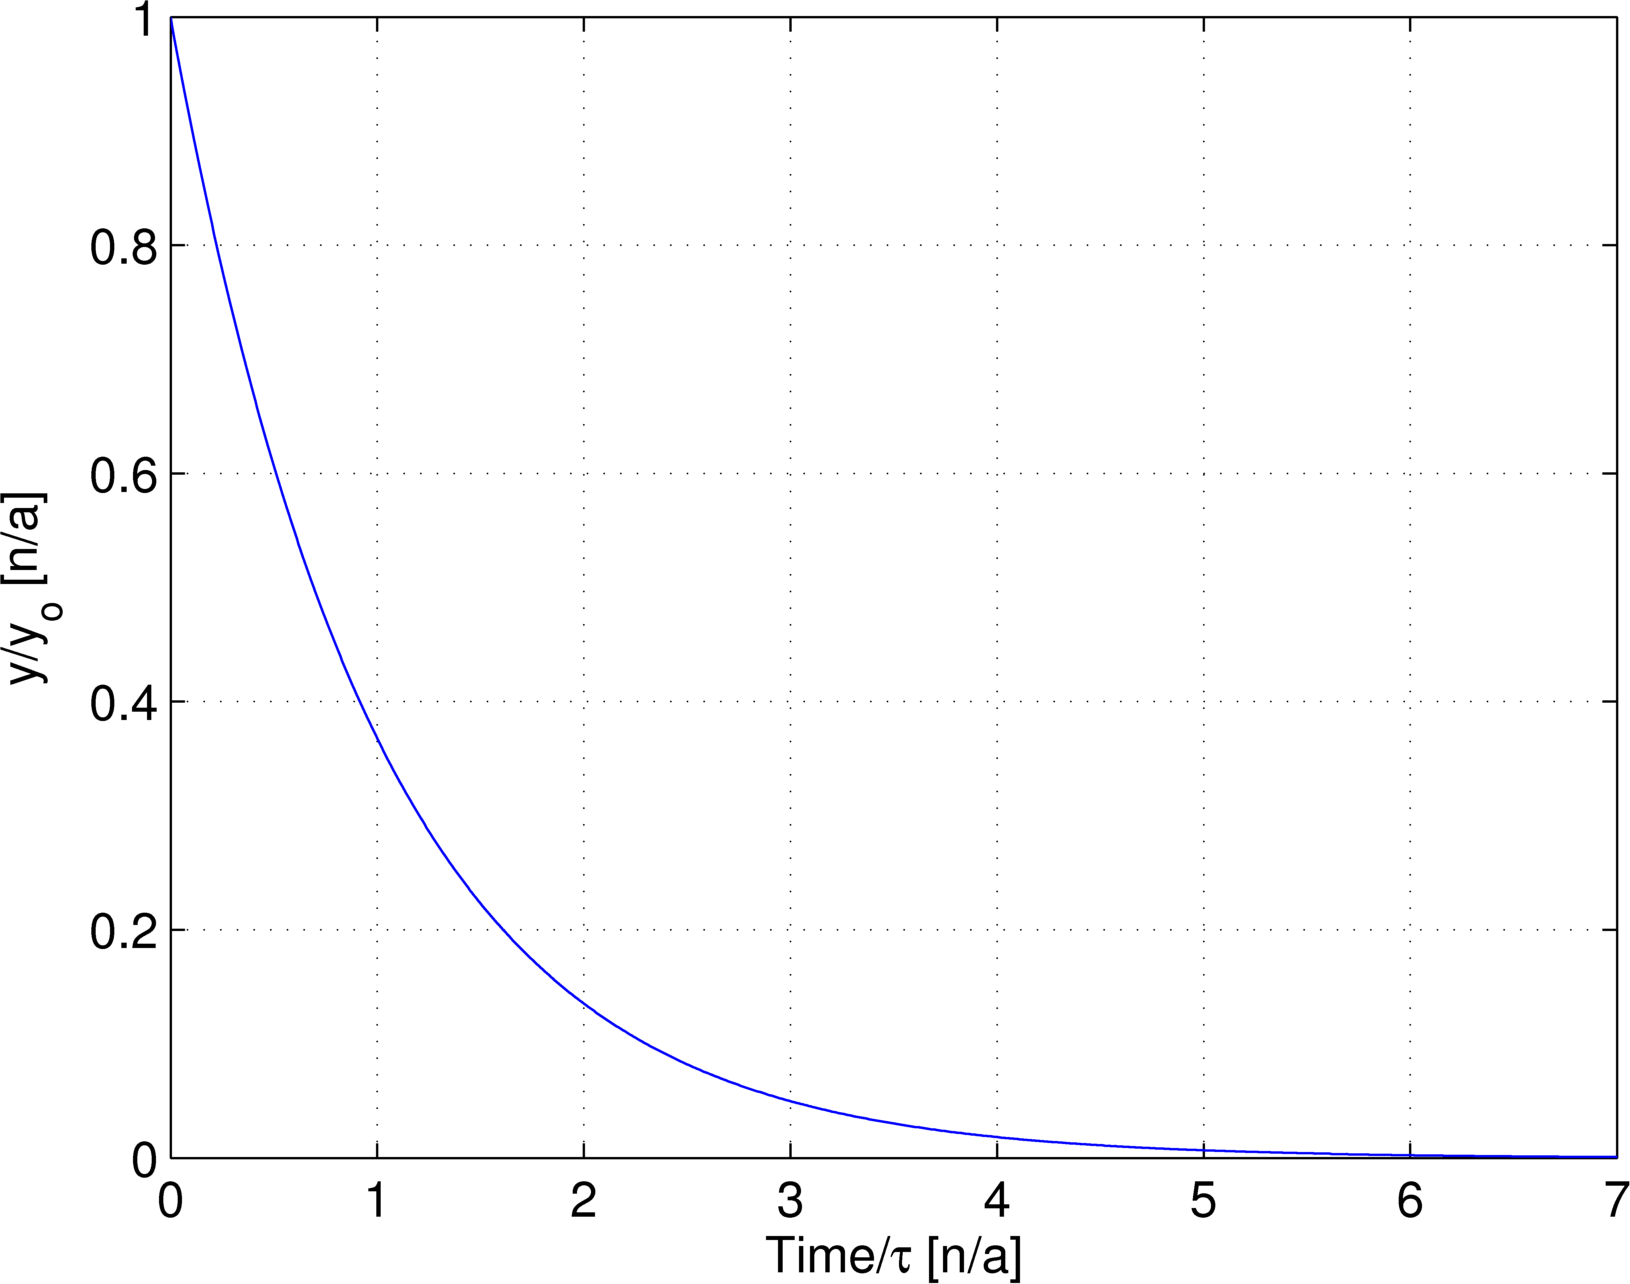
\includegraphics[width=\FigWidth\textwidth]{firstfree.png}
\caption{Graph of the free response (\ref{e:firstfree}).  Notice that the $x$ and $y$ axes have been normalized so that the output is the ratio of the response and the initial condition and the time is the ratio of time and the time constant.}
\label{f:firstfree}
\end{figure}

\begin{ex}
Using our automobile model (\ref{e:car}), write an expression for the free response of this model with appropriate physical parameters.  Create a graph of the free response with the initial condition $v(0)=\unit[60]{mph}$. For the x-axis of the graph use the units mph and for the y-axis of the graph use the units seconds.
\end{ex}

